\documentclass{article}
\usepackage{tikz}
\usetikzlibrary{arrows.meta}
\title{Graphs with Tikz}
\author{Sumaiya Tabassum}

\begin{document}

	\maketitle
	\tableofcontents
	\clearpage
	
	\section{Nodes:}
		\subsection{Normal Node:}
			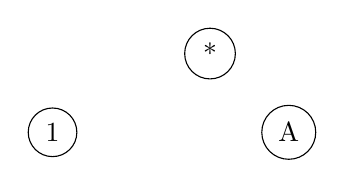
\begin{tikzpicture}
				\node(1) at (0,0) [circle,draw]{1};
				\node(2) at (2,1) [circle,draw]{*};
				\node(3) at (3,0)[circle,draw]{A};
			\end{tikzpicture}
			
		\subsection{Normal Nodes with various shapes:}
			\begin{tikzpicture}
				\node(1) at (0,0)[circle, draw]{1};
				
				\node(2) at (5,0)[draw]{2};
			\end{tikzpicture}
			
		\subsection{Normal Nodes with filled color and face color:}
		% For Fill color: \node(serial_of_node) at(x,y)[circle,color_name,draw]{name_of node}
	%For Face colore:  \node(serial_of_node) at(x,y)[circle,fill=color_name,draw]{name_of node}
	% For face and Fill at time: \node(serial_of_node) at(x,y)[circle,color_name,fill=color_name,draw]{name_of node}
			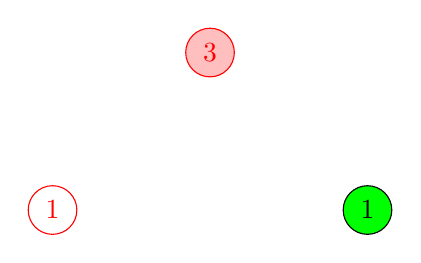
\begin{tikzpicture}
				\node(1) at (0,0) [circle,red,draw]{1};
				\node(2) at (4,0) [circle,fill=green,draw]{1};
				\node(3) at (2,2)[circle,red,fill=pink,draw]{3};
			\end{tikzpicture}
			
		\subsection{A solid node with outside title:}
		%we can use: label=left/right/below/above
	% for size= inner spp= valuept
	%For Text color: text=color_name
			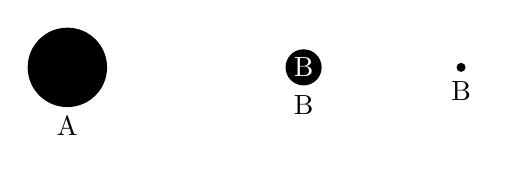
\begin{tikzpicture}
				\node(1) at (0,0)[circle,fill=black,text=white,inner sep=10pt,label=below:A,draw]{};
				\node(2) at (3,0)[circle,fill=black,text=white,inner sep=1pt,label=below:B,draw]{B};
				\node(3) at (5,0)[circle,fill=black,text=white,inner sep=1pt,label=below:B,draw]{};
				
			\end{tikzpicture}
			
			
	\section{Edges:}
		\subsection{Normal edge between two or more nodes:}
			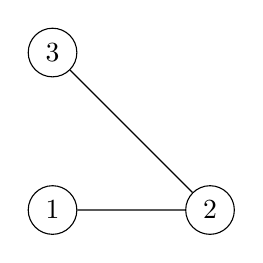
\begin{tikzpicture}
				\node(1) at (0,0)[circle,draw]{1};
				\node(2) at (2,0)[circle,draw]{2};
				\node(3) at (0,2)[circle,draw]{3};
				\draw(1) to (2) -- (3);		
			\end{tikzpicture}
			
		\subsection{Normal edge with arrow and color between two or among more nodes:}
			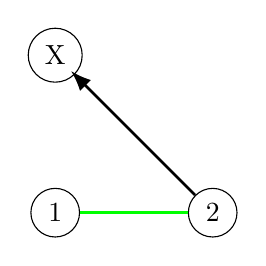
\begin{tikzpicture}
				\node(1) at (0,0)[circle,draw]{1};
				\node(2) at (2,0)[circle,draw]{2};
				\node(3) at (0,2)[circle,draw]{X};
				\draw[-,very thick,green](1)--(2);	
				%\usetikzlibrary{arrows.meta}
				\draw[->, >=Latex, line width=1pt, shorten >=-2pt](2) to (3);	
			\end{tikzpicture}
			
		\subsection{Curved edge with arrow between two or among more node:}
		%Create: upward curved edge:  \draw[->, bend left=angle] (starting_node) to (ending_node);
	%Create: downward curved edge:  \draw[->, bend right=angle] (starting_node) to (ending_node);
			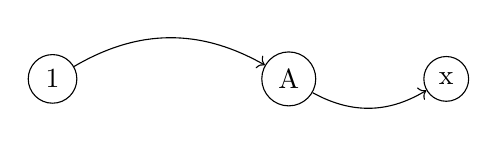
\begin{tikzpicture}
				\node(1) at (0,0)[circle,draw]{1};
				\node(2) at (3,0) [circle,draw]{A};
				\node(3) at (5,0)[circle ,draw]{x};
				\draw[->,bend left=30](1) to (2);	
				\draw[->,bend right=30](2) to (3);			\end{tikzpicture}			
			
		\subsection{Self loop in any node:}
			\begin{tikzpicture}
				\node(1) at (0,0)[circle,draw]{1};
				\draw[->,loop above](1) to (1);	
				\node(2) at (5,0)[circle,draw]{2};
				\draw[->,loop right](2) to (2);	
			\end{tikzpicture}
			
	\section{Practice:}
		\subsection{Practice 01:}
			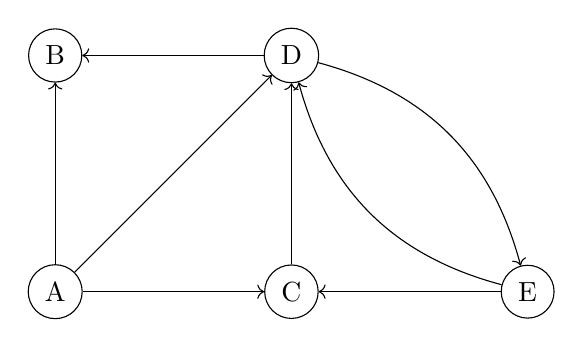
\begin{tikzpicture}
				\node(B) at (0,0)[circle,draw]{B};
				\node(D) at (3,0)[circle,draw]{D};
				\node(A) at (0,-3)[circle,draw]{A};
				\node(C) at (3,-3)[circle,draw]{C};
				\node(E) at (6,-3)[circle,draw]{E};
				
				\draw[->] (A) to (B);
				\draw[->] (D) to (B);
				\draw[->] (A) to (D);
				\draw[->] (A) to (C);
				\draw[->] (E) to (C);
				\draw[->] (C) to (D);
				\draw[->, bend left=30] (D) to (E);
				\draw[->, bend left=30] (E) to (D);
			\end{tikzpicture}
			
		\subsection{Practice 01:}
			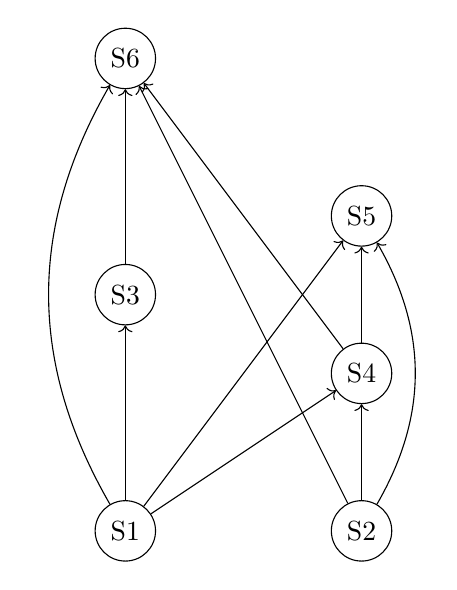
\begin{tikzpicture}
				\node(s6) at (0,0)[circle,draw]{S6};
				\node(s3) at (0,-3)[circle,draw]{S3};
				\node(s1) at (0,-6)[circle,draw]{S1};
				\node(s5) at (3,-2)[circle,draw]{S5};
				\node(s4) at (3,-4)[circle,draw]{S4};
				\node(s2) at (3,-6)[circle,draw]{S2};
				
				\draw[->] (s1) to (s3);
				\draw[->] (s1) to (s4);
				\draw[->] (s1) to (s5);
				\draw[->] (s2) to (s6);
				\draw[->] (s4) to (s6);
				\draw[->] (s3) to (s6);
				\draw[->] (s2) to (s4);
				\draw[->] (s4) to (s5);
				\draw[->, bend left = 30] (s1) to (s6);
				\draw[->, bend right = 30] (s2) to (s5);
				
			\end{tikzpicture}
			
		\subsection{Practice 02:}
			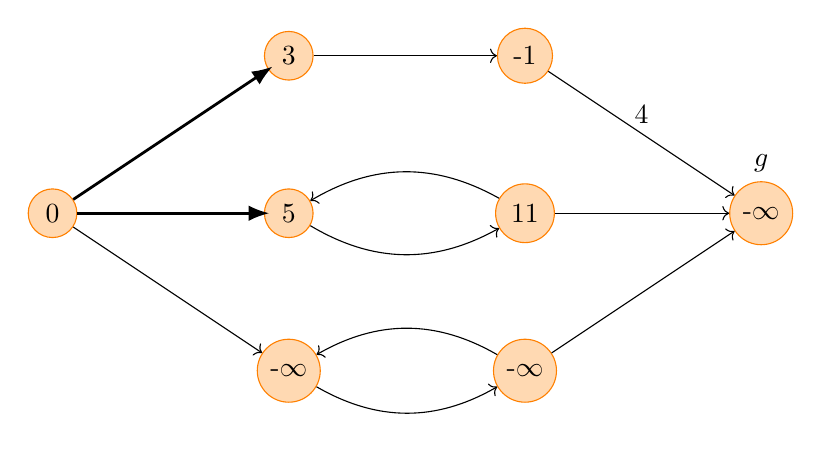
\begin{tikzpicture}
				\node(0) at (0,0)[circle,orange,fill= orange!30,text=black,draw]{0};
				\node(3) at (3,2)[circle,orange,fill= orange!30,text=black,draw]{3};
				\node(5) at (3,0)[circle,orange,fill= orange!30,text=black,draw]{5};
				\node(i1) at (3,-2)[circle,orange,fill= orange!30,text=black,draw]{-$\infty$};
				\node(-1) at (6,2)[circle,orange,fill= orange!30,text=black,draw]{-1};
				\node(11) at (6,0)[circle,orange,fill= orange!30,text=black,draw]{11};
				\node(i2) at (6,-2)[circle,orange,fill= orange!30,text=black,draw]{-$\infty$};
				\node(i3) at (9,0)[circle,orange,fill= orange!30,text=black,label=above:$g$,draw]{-$\infty$};
%\usetikzlibrary{arrows.meta}
				\draw[->, >=Latex, line width=1pt, shorten >=-2pt] (0) to (3);
				\draw[->, >=Latex, line width=1pt, shorten >=-2pt] (0) -- (5);
				\draw[->] (0) to (i1);
				\draw[->] (3) to (-1);
				\draw[->, bend right =30] (5) to (11);
				\draw[->,bend right =30] (11) to (5);
				\draw[->, bend right =30] (i1) to (i2);
				\draw[->,bend right =30] (i2) to (i1);
				\draw[->] (-1) to  node[midway, above]{4}(i3);
				\draw[->] (11) to (i3);
				\draw[->] (i2) to (i3);
				
			\end{tikzpicture}

\end{document}